\documentclass[11pt,a4paper]{article}
\usepackage[utf8]{inputenc}
\usepackage{amsmath}
\usepackage{amsfonts}
\usepackage{graphicx}
\usepackage[table,xcdraw]{xcolor}


\usepackage{caption}
\usepackage{subcaption}

\renewcommand{\familydefault}{\sfdefault} % cambiamos la fuente a una sans

\usepackage{float} % para que floten las imagenes o algo asi...
\usepackage{wallpaper} %paquete para usar una imagen como encabezado!
\usepackage{hyperref} %para usar hypervinculos 
\usepackage[export]{adjustbox} %para usar marcos en imagenes
\usepackage{eurosym} % para el euro
\usepackage{transparent} %para las marcas de agua
\usepackage{eso-pic}  %para las marcas de agua

\definecolor{azul_marcos}{RGB}{0,128,159} %defino el color azul de los marcos
\usepackage{sectsty} %esto es para cambiar el color de las fuentes creo
\renewcommand{\familydefault}{\sfdefault} % cambiamos la fuente a una sans
\sectionfont{\color{azul_marcos}}  % sets colour of sections
\subsectionfont{\color{azul_marcos}}  % sets colour of sections


\usepackage{pdfpages} %para insertar pdfs
\usepackage{amssymb}
\usepackage{pstcol} % para color
\usepackage{pst-node} % para diagramas
\usepackage{pst-plot} % para representacion de dat
\usepackage[spanish]{babel}
\addto\captionsspanish{\renewcommand\chaptername{Bloque}}
%\usepackage[total={18cm,21cm},top=2cm, left=2cm]{geometry}
\usepackage{anysize}
\pagestyle{plain}
%\markboth{left head}{right head}
%\markright{Guía de impresión FlexiSMART}
\marginsize{3cm}{2cm}{2.5cm}{1cm}
\title{Guía de impresión FlexiSMART}
\date{}

%configuracion de la marca de agua
\AddToShipoutPicture{
    \put(0,0){
        \parbox[b][\paperheight]{\paperwidth}{%
            \vfill
            \centering
            {\transparent{0.2}
\includegraphics[scale=1.25]{FOTOS/logofff}}%
            \vfill
        }
    }
}

\begin{document}
\ULCornerWallPaper{1}{FOTOS/header}
\LLCornerWallPaper{1}{FOTOS/footer}
%\maketitle
\tableofcontents

\includepdf{PDF/ES_PORTADA.pdf}
\section{¿Qué es FlexiSMART?}FlexiSMART es un filamento para impresión 3D FFF/FDM fabricado a partir de polímeros elastómeros termoplásticos (TPE) con aditivos químicos para hacerlo más fácil de imprimir por la mayoría de impresoras 3D del mercado.
\\\\
FlexiSMART es flexible y recupera su forma al doblarlo, retorcerlo o estirarlo.

\section{¿Por qué usar FlexiSMART?}
FlexiSMART te permite adentrarte en un nuevo mundo de posibilidades gracias a la naturaleza flexible del filamento. A partir de ahora puedes imprimir objetos que antes con un filamento rígido no podías: Fundas de smartphones, tablets, zapatillas, plantillas, ruedas de RC, prótesis, silent blocks, engranajes que necesiten cierta adaptabilidad, y en general, cualquier objeto que se te ocurra y pueda hacer uso de sus propiedades.
\\\\
FlexiSMART ha sido diseñado para ser fácil de imprimir:
\begin{itemize}
\item Tiene cierta rigidez para que pueda ser impreso por la mayoría de extrusores directos haciendo ninguna o pocas modificaciones.
\item La adherencia es excelente. Puedes imprimirlo incluso sin cama caliente.
\item La resistencia es muy alta, por lo que las piezas impresas no se degradarán rápido.
\item Es el filamento flexible con los precios más atractivos de Europa.
\end{itemize}

\section{Ficha técnica y parámetros de impresión}

\begin{table}[H]
\centering
\caption*{Ficha técnica}
\begin{tabular}{|
>{\columncolor[HTML]{FFFFFF}}l |
>{\columncolor[HTML]{FFFFFF}}c |}
\hline
\multicolumn{1}{|c|}{\cellcolor[HTML]{FFFFFF}\textbf{Material}}   & FlexiSMART (TPE)   \\ \hline
\textbf{Colores disponibles}              & 11                 \\ \hline
\textbf{Formatos disponibles}             & 1kg, 250gr         \\ \hline
\textbf{Temperatura de deflexión térmica} & 90ºC               \\ \hline
\textbf{Temperatura de fusión}            & 160ºC              \\ \hline
\textbf{Temperatura de descomposición}    & \textgreater 240ºC \\ \hline
\textbf{Densidad}                         & 0.96 gr / cm3      \\ \hline
\textbf{Estiramiento máximo}              & 600\%              \\ \hline
\end{tabular}
\end{table}
\begin{table}[H]
\centering
\caption*{Parámetros de impresión recomendados usando un nozzle de 0.4 mm}
\begin{tabular}{|
>{\columncolor[HTML]{FFFFFF}}l |
>{\columncolor[HTML]{FFFFFF}}c |}
\hline
\multicolumn{1}{|c|}{\cellcolor[HTML]{FFFFFF}\textbf{Temperatura recomendada de impresión}} & 195º-220º              \\ \hline
\textbf{Velocidad recomendada de impresión}                         & 20-60mm/s              \\ \hline
\textbf{Temperatura cama caliente}                                  & \textgreater 18º        \\ \hline
\textbf{Altura de capa óptima}                                      & 0.2 mm                 \\ \hline
\textbf{Perímetros}                                                 & 3                      \\ \hline
\textbf{Top solid layers}                                           & 5                      \\ \hline
\textbf{Retracción}                                                 & Desactivada o reducida \\ \hline
\end{tabular}
\end{table}

Puedes descargarte nuestros perfiles completos de impresión de los principales programas de laminación (Cura, Slic3r y Simplify3D) desde nuestra página web:
\\\\
\centerline{ {\huge \url{www.fffworld.com/documentation} } }
\\\\
Los parámetros óptimos dependerán de la impresora 3D que utilices, sin embargo, son unos buenos parámetros para tenerlos como punto de partida. Con unas pocas impresiones serás capaz de encontrar los límites y la configuración perfecta para tu maquina.
\section{Problemas y soluciones}
	\subsection{Problemas al extruir FlexiSMART}
El principal reto a la hora de imprimir FlexiSMART y otros filamentos flexibles deriva de la propia naturaleza del material ya que, al ser flexible, no puede ser empujado con la misma facilidad que los materiales rígidos, de la misma manera que no se puede empujar una cuerda.
\\\\
El problema se da cuando hay holguras en ciertas partes del extrusor, en particular, entre la drive-gear (la rueda dentada que empuja el filamento) y el orificio a través del cual el filamento accede al hot-end (punta metálica que funde el filamento).
\\\\
Cuando este espacio es lo suficientemente grande el filamento tiende a salirse de su recorrido y a formar un nudo que termina asomando por un lateral del extrusor, como puede verse en la imagen.
\begin{figure}[H]
\centering
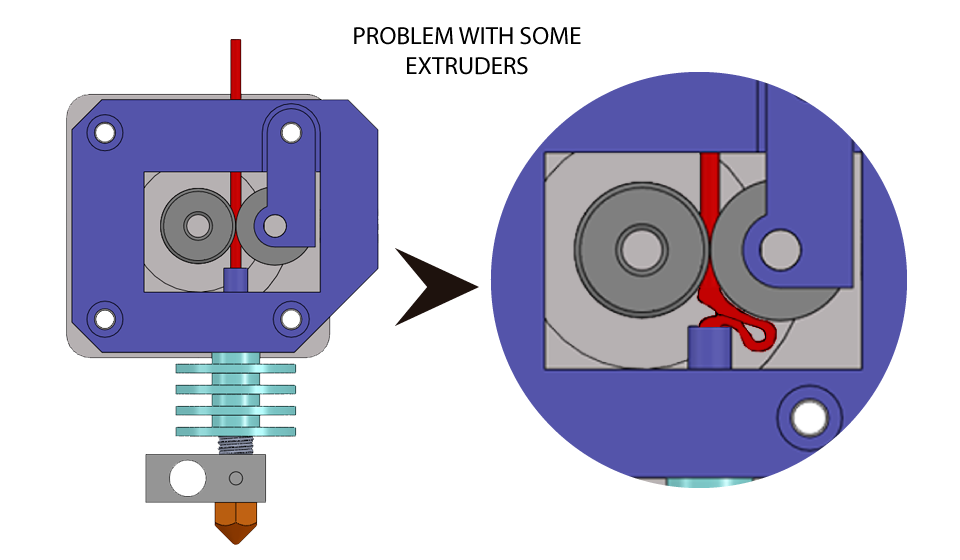
\includegraphics[width=0.5\textwidth,cfbox=azul_marcos 4pt 0pt]{FOTOS/NUDOS1}
\caption*{Extrusor NO optimizado para filamentos flexibles}
\end{figure}
Este problema es mayor al usar filamento de 1.75 mm ya que al tener menos sección es aún más propenso a salirse de su recorrido.
\\\\
La velocidad de extrusión es determinante en la aparición de este problema. Si el extrusor trata de empujar el filamento a demasiada velocidad se crea una presión hacia arriba que hace que el filamento se salga de su camino natural. Por ello la recomendación general es comenzar imprimiendo a una velocidad baja o muy baja e ir incrementándola hasta encontrar la máxima velocidad que soporta tu extrusor. El tamaño del nozzle también afecta a la velocidad máxima soportada ya que cuanto más grande sea éste más material fundido podrá extruirse por unidad de tiempo y, por tanto, mayor será la velocidad a la que se pueda hacer.
\\\\
Los extrusores diseñados para utilizar filamentos flexibles minimizan las holguras impidiendo que el filamento pueda salirse e incorporan un sistema de doble drive-gear para canalizar con precisión el filamento y evitar completamente el problema mencionado al tiempo que permiten aumentar la velocidad de impresión.
\begin{figure}[H]
\centering
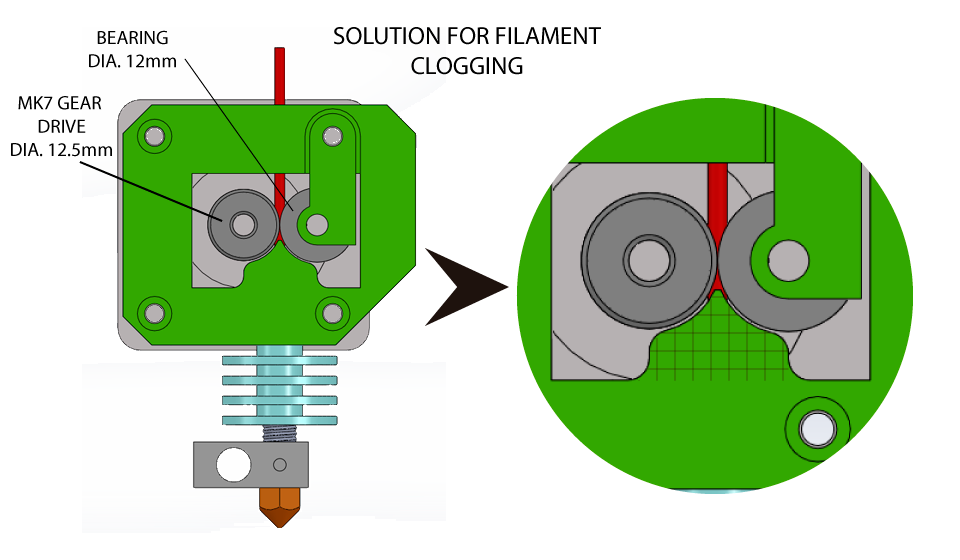
\includegraphics[width=0.5\textwidth,cfbox=azul_marcos 4pt 0pt]{FOTOS/NUDOS2}
\caption*{Extrusor optimizado para filamentos flexibles}
\end{figure}
\emph{FlexiSMART ha sido diseñado pensando en estos problemas y tiene una rigidez superior a otros filamentos flexibles para ayudar a reducirlos.}
\\\\
No obstante en extrusores que no están diseñados para usar materiales elásticos estos problemas puede aparecer.
	\subsection{Preparando el extrusor para imprimir FlexiSMART}Si estás teniendo alguno de los problemas anteriormente mencionados probablemente tengas que adaptar o sustituir tu extrusor. En este sentido existen varias opciones que detallamos a continuación.
		\subsubsection{Modificar tu extrusor}
En ocasiones es posible utilizar FlexiSMART en extrusores no optimizados realizando algunas modificaciones sobre el mismo extrusor.
\\\\
Si estás teniendo problemas para imprimir FlexiSMART te sugerimos que sigas los siguientes consejos, expuestos en orden de complejidad.
			\paragraph{Limar el conducto por el que el filamento accede al hot-end}\mbox{}\\\\
Si usas un extrusor con el cuerpo de plástico, como los extrusores imprimibles, te recomendamos que pruebes lo siguiente. 
\\\\
Lima ligeramente los bordes del orificio que se encuentra justo debajo de la drive-gear, orificio a través del cual se canaliza el filamento hacia el hot-end. Esto permite evitar rozamientos y enganches que pueden provocar los nudos anteriormente descritos. 
\\\\
Puede ser necesario desmontar parte del extrusor para realizar esta operación.
			\paragraph{Insertar tubo de teflón en el extrusor}\mbox{}\\\\
Una segunda opción, más complicada pero más efectiva, es insertar un tubo de teflon (PTFE) en el mencionado orificio. Esta técnica además permite reducir el espacio con la drive-gear ya que dicho tubo puede colocarse muy próximo a aquella. Incluso se puede modificar la entrada del tubo de teflón para adaptarlo a la forma del drive-gear dejando un espacio mínimo.
\\\\
En general esta técnica implica taladrar el extrusor para permitir la inserción del mencionado tubo de teflón. A continuación puedes ver unas imágenes del resultado:
\begin{figure}[H]
    \centering
    \begin{subfigure}[b]{0.3\textwidth}
        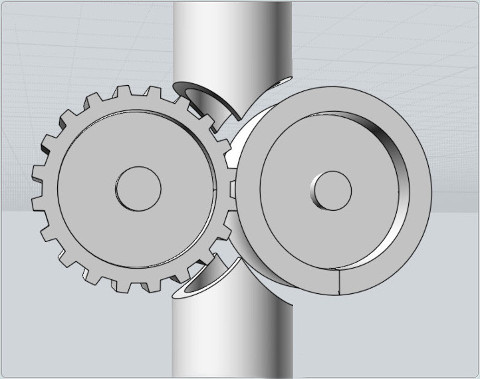
\includegraphics[width=\textwidth,cfbox=azul_marcos 4pt 0pt]{FOTOS/TEFLON1}
    \end{subfigure}
    ~ %add desired spacing between images, e. g. ~, \quad, \qquad, \hfill etc. 
      %(or a blank line to force the subfigure onto a new line)
    \begin{subfigure}[b]{0.3\textwidth}
        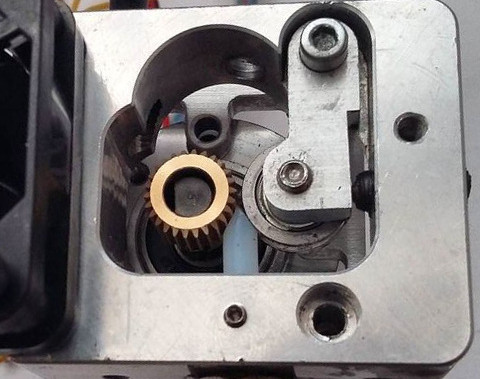
\includegraphics[width=\textwidth,cfbox=azul_marcos 4pt 0pt]{FOTOS/TEFLON2}
    \end{subfigure}
    ~ %add desired spacing between images, e. g. ~, \quad, \qquad, \hfill etc. 
    %(or a blank line to force the subfigure onto a new line)
    \begin{subfigure}[b]{0.3\textwidth}
        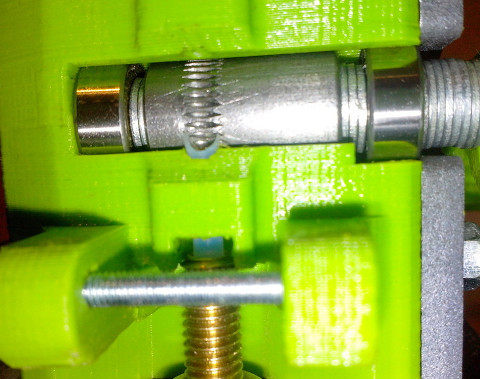
\includegraphics[width=\textwidth,cfbox=azul_marcos 4pt 0pt]{FOTOS/TEFLON3}
    \end{subfigure}
    \caption*{Injertos de teflón}
\end{figure}
			\paragraph{Imprimir una guía para el filamento y colocarla en el extrusor}\mbox{}\\\\
La tercera opción es imprimir una pieza que haga de guía para el filamento y colocarla debajo del drive-gear. Estas piezas suelen tener una forma triangular y deben estar diseñadas respetando las dimensiones de cada extrusor.
\\\\
En internet, en sitios como \url{www.thingiverse.com}, se pueden descargar este tipo de adaptadores para algunos de los extrusores más habituales. No obstante se trata de un diseño sencillo que aquellos con conocimientos de diseño 3D podrán crear desde cero con facilidad.
\begin{figure}[H]
    \centering
    \begin{subfigure}[b]{0.5\textwidth}
        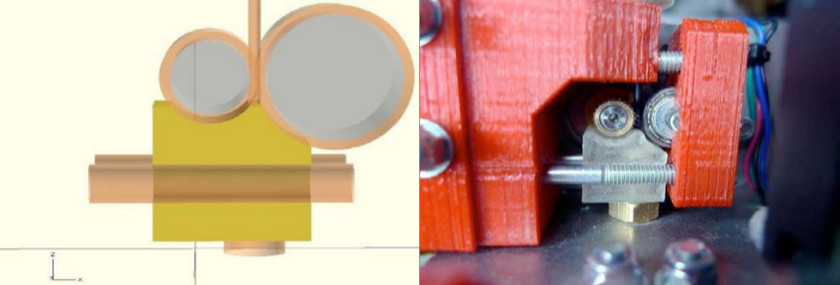
\includegraphics[width=\textwidth,cfbox=azul_marcos 4pt 0pt]{FOTOS/GUIA1}
    \end{subfigure}
    ~ %add desired spacing between images, e. g. ~, \quad, \qquad, \hfill etc. 
      %(or a blank line to force the subfigure onto a new line)
    \begin{subfigure}[b]{0.5\textwidth}
        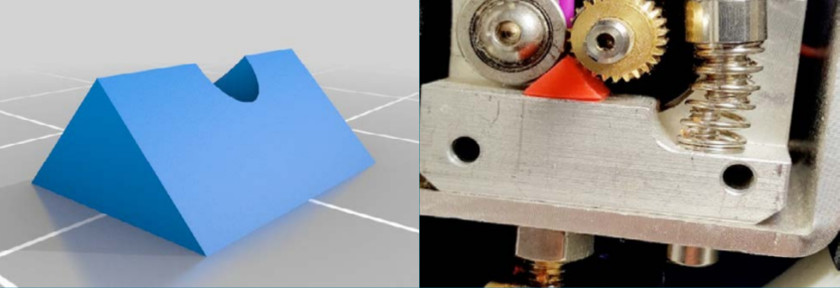
\includegraphics[width=\textwidth,cfbox=azul_marcos 4pt 0pt]{FOTOS/GUIA2}
    \end{subfigure}
    ~ %add desired spacing between images, e. g. ~, \quad, \qquad, \hfill etc. 
    %(or a blank line to force the subfigure onto a new line)
    \begin{subfigure}[b]{0.5\textwidth}
        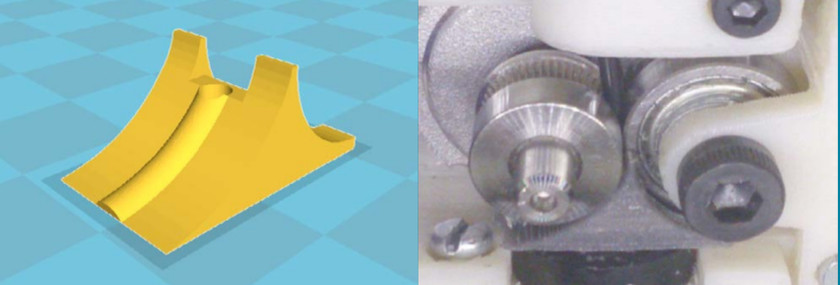
\includegraphics[width=\textwidth,cfbox=azul_marcos 4pt 0pt]{FOTOS/GUIA3}
    \end{subfigure}
    \caption*{Guías de filamento imprimibles}
\end{figure}	

	\paragraph{Ajustando la presión del drive-gear sobre el filamento}\mbox{}\\\\
Al tratarse de un material flexible es especialmente importante que la presión del mecanismo que empuja el filamento hacia el hot-end no sea excesiva. En los filamentos rígidos un exceso de presión producirá pequeñas muescas en su superficie pero en el caso de FlexiSMART una presión excesiva deforma la sección del filamento dándole una forma ovalada que hace que se vuelva propenso a atascar el extrusor.
\\\\
Los extrusores diseñados para la impresión de filamentos flexibles tienen esto en cuenta y disponen de un mecanismo para regular la presión del mecanismo tractor. Si tu extrusor permite regular dicha presión te recomendamos que la ajustes al utilizar FlexiSMART. La presión adecuada será la mínima necesaria que permita que el extrusor mueva el filamento.
\\\\
Si tu extrusor no dispone de mecanismo para regular la presión, aún puedes reducirla cambiando el muelle o reduciendo el recorrido posible mediante la colocación de una cuña en el lugar preciso. A modo de ejemplo te mostramos una imagen de cómo reducir la presión en un extrusor que no está preparado para ello:
\begin{figure}[H]
\centering
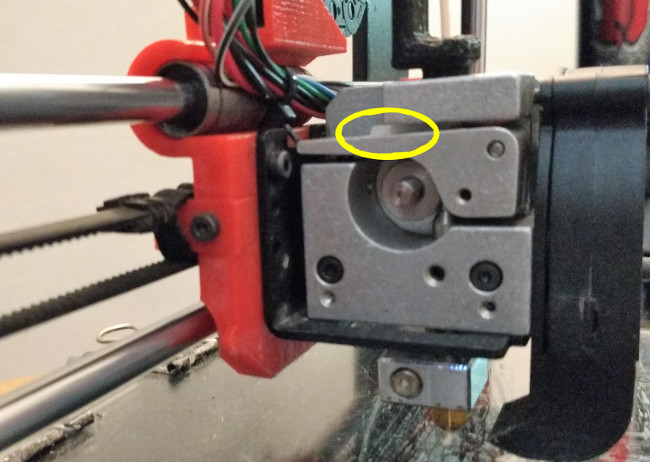
\includegraphics[width=0.5\textwidth,cfbox=azul_marcos 4pt 0pt]{FOTOS/SOLUCION1}
\caption*{HeatCore Extruder de BQ Hephestos y BQ Witbox}
\end{figure}
			\paragraph{Añadiendo tensión entre la bobina y el extrusor}\mbox{}\\\\
Se ha comprobado que en algunos modelos de impresora es conveniente que al utilizar filamento flexible exista algo de tensión entre la bobina y el extrusor de forma que el filamento no quede colgando.
\\\\
Para conseguirlo puedes tratar de frenar la bobina de manera que el extrusor tenga que tirar ligeramente del filamento para desenrollarlo. También puedes colocar un accesorio similar al de la fotografía para alcanzar el mismo objetivo.
\begin{figure}[H]
\centering
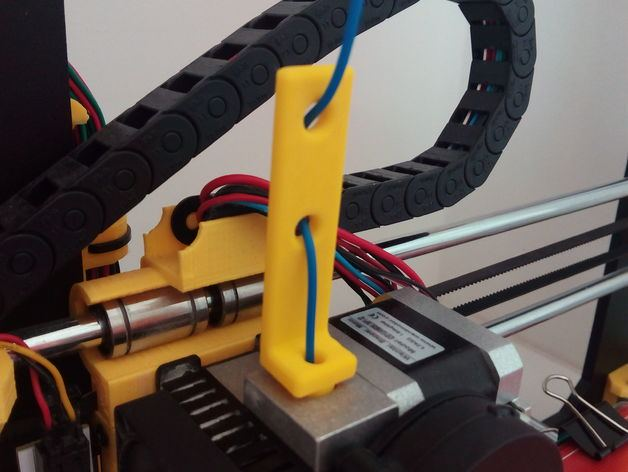
\includegraphics[width=0.5\textwidth,cfbox=azul_marcos 4pt 0pt]{FOTOS/SOLUCION2}
\caption*{Diseñado para Extrusor BQ Unibody de BQ Hephestos}
\end{figure}
		\subsubsection{Sustituir tu extrusor por uno optimizado}
Hoy en día los filamentos flexibles se han hecho populares hasta el punto de que es dificil que una impresora de última generación no esté preparada para imprimirlos.
\\\\
Además son muchos los diseñadores que han creado extrusores imprimibles capaces de imprimir FlexiSMART y otros filamentos. Estos extrusores pueden descargarse desde páginas como Thingiverse para ser impresos y ensamblados en casa.
\\\\
También son cada vez más los extrusores comerciales preparados para imprimir filamentos flexibles que pueden adquirirse y montarse en nuestras impresoras.
			\paragraph{Extrusores imprimibles DIY}\mbox{}\\\\
Algunos de estos extrusores están diseñados desde cero y otros son modificaciones realizadas sobre diseños ya existentes. Aquí presentamos una lista no exhaustiva de diseños de extrusores que pueden ser descargados desde internet. Siguiendo cada enlace podrás encontrar la lista de componentes completa así como instrucciones de montaje y comentarios de otros usuarios.
\\\\
El hot-end que instale en su extrusor debe tener una pieza de teflón (PTFE) en su interior para evitar fricciones y que FlexiSMART se imprima correctamente. FlexiSMART ha sido probado con éxito en los siguientes hot-ends\footnote{Debes tener en cuenta que dichas pruebas han sido realizadas con hot-ends originales y no podemos garantizar el mismo resultado en réplicas de éstos.}:
\begin{itemize}
\item J-Head MKV-B
\item Budassnozzle V1.3
\item E3D v6
\item Leonnozzle V2
\end{itemize}
Dependiendo de qué impresora utilices, algunos de estos extrusores serán más fáciles de instalar puesto que podrán reemplazar directamente al extrusor original de la máquina.
\begin{figure}[H]
    \centering
    \begin{subfigure}[b]{0.4\textwidth}
        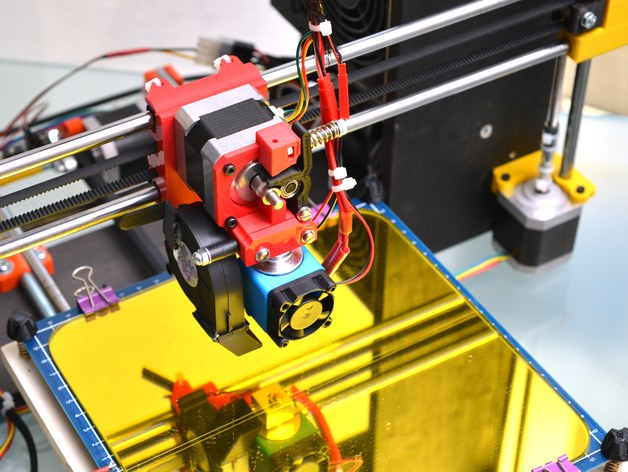
\includegraphics[width=\textwidth,cfbox=azul_marcos 4pt 0pt]{FOTOS/EXTRUSOR1}
		\caption*{\href{http://www.thingiverse.com/thing:147705}{{\footnotesize Direct-drive hinged extruder for E3D/J-Head hot-end (Prusa i3) by ffleury}}}
    \end{subfigure}
    ~ \qquad%add desired spacing between images, e. g. ~, \quad, \qquad, \hfill etc. 
      %(or a blank line to force the subfigure onto a new line)
    \begin{subfigure}[b]{0.4\textwidth}
        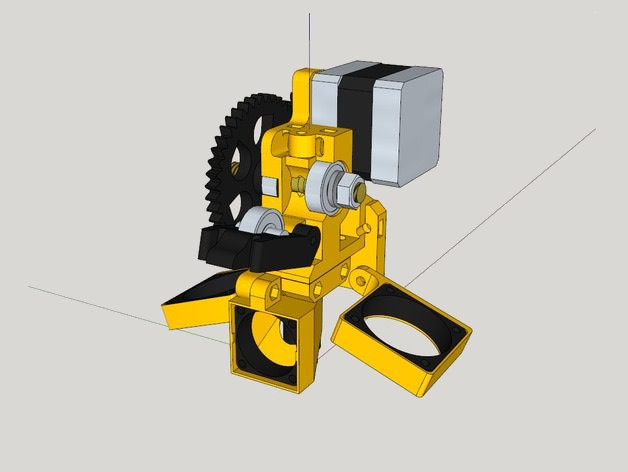
\includegraphics[width=\textwidth,cfbox=azul_marcos 4pt 0pt]{FOTOS/EXTRUSOR2}
		\caption*{\href{http://www.thingiverse.com/thing:512338}{{\footnotesize Wade L3K Extruder (prusa I3) compatible filament flexible By Skarab}}}
    \end{subfigure}
\end{figure}
\begin{figure}[H]
    \centering
    ~ %add desired spacing between images, e. g. ~, \quad, \qquad, \hfill etc. 
    %(or a blank line to force the subfigure onto a new line)
    \begin{subfigure}[b]{0.4\textwidth}
        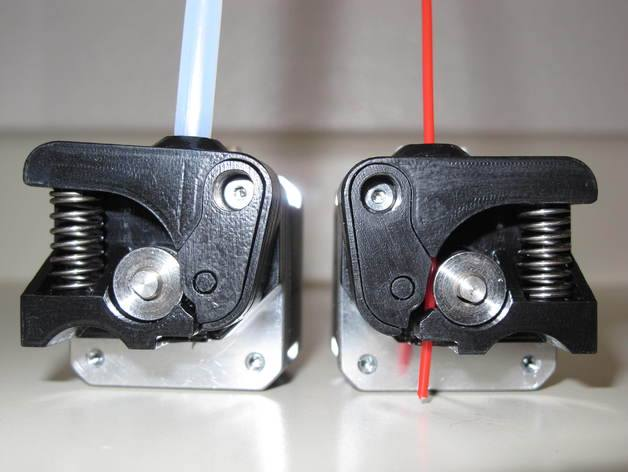
\includegraphics[width=\textwidth,cfbox=azul_marcos 4pt 0pt]{FOTOS/EXTRUSOR3}
		\caption*{\href{http://www.thingiverse.com/thing:403438}{{\footnotesize Printrbot Flexible Filament Direct Drive Extruder by thirdhorizon}}}
    \end{subfigure}
    ~ \qquad %add desired spacing between images, e. g. ~, \quad, \qquad, \hfill etc. 
    %(or a blank line to force the subfigure onto a new line)
    \begin{subfigure}[b]{0.4\textwidth}
        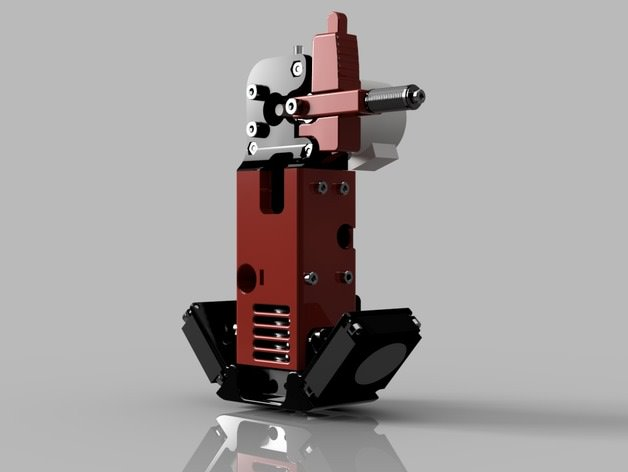
\includegraphics[width=\textwidth,cfbox=azul_marcos 4pt 0pt]{FOTOS/EXTRUSOR4}
		\caption*{\href{http://www.thingiverse.com/thing:1102900}{{\footnotesize Ultimaker 2 PG35L Direct Drive Extruder for 1.75mm E3D v6 Hotend by jasonatepaint}}}
    \end{subfigure}
\end{figure}
			\paragraph{Extrusores comerciales}\mbox{}\\\\
Adquirir un extrusor comercial es más caro que construir uno casero sin embargo, suelen dar mejor rendimiento que éstos y son la mejor opción cuando se va a usar filamento flexible de forma intensiva.
\\\\
Estos extrusores han sido específicamente diseñados para evitar todos los problemas mencionados anteriormente y algunos pueden extruir FlexiSMART a velocidades superiores a los 70 mm/s.
\begin{figure}[H]
    \centering
    \begin{subfigure}[b]{0.4\textwidth}
        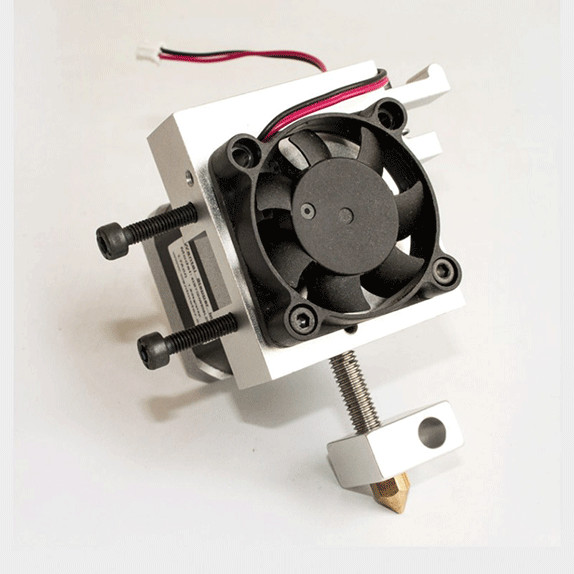
\includegraphics[width=\textwidth,cfbox=azul_marcos 4pt 0pt]{FOTOS/EXTRUSOR5}
		\caption*{\href{http://www.recreus.com}{{\footnotesize Recreus Extruder - Precio aprox. 100\euro}}}
    \end{subfigure}
    ~ \qquad%add desired spacing between images, e. g. ~, \quad, \qquad, \hfill etc. 
      %(or a blank line to force the subfigure onto a new line)
    \begin{subfigure}[b]{0.4\textwidth}
        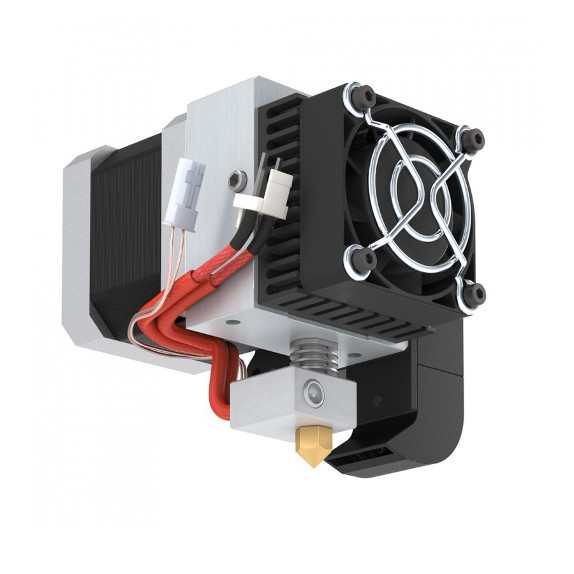
\includegraphics[width=\textwidth,cfbox=azul_marcos 4pt 0pt]{FOTOS/EXTRUSOR6}
		\caption*{\href{http://www.bq.es}{{\footnotesize BQ HeatCore DDG Extruder - Precio 140\euro}}}
    \end{subfigure}
\end{figure}
\begin{figure}[H]
    \centering
    ~ %add desired spacing between images, e. g. ~, \quad, \qquad, \hfill etc. 
    %(or a blank line to force the subfigure onto a new line)
    \begin{subfigure}[b]{0.4\textwidth}
        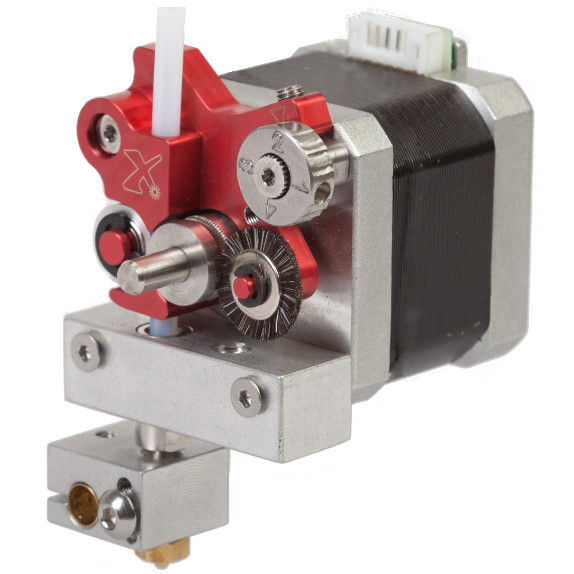
\includegraphics[width=\textwidth,cfbox=azul_marcos 4pt 0pt]{FOTOS/EXTRUSOR7}
		\caption*{\href{https://flexionextruder.com/}{{\footnotesize Flexion Extruder - Precio aprox. 140\euro}}}
    \end{subfigure}
    ~ \qquad %add desired spacing between images, e. g. ~, \quad, \qquad, \hfill etc. 
    %(or a blank line to force the subfigure onto a new line)
    \begin{subfigure}[b]{0.4\textwidth}
        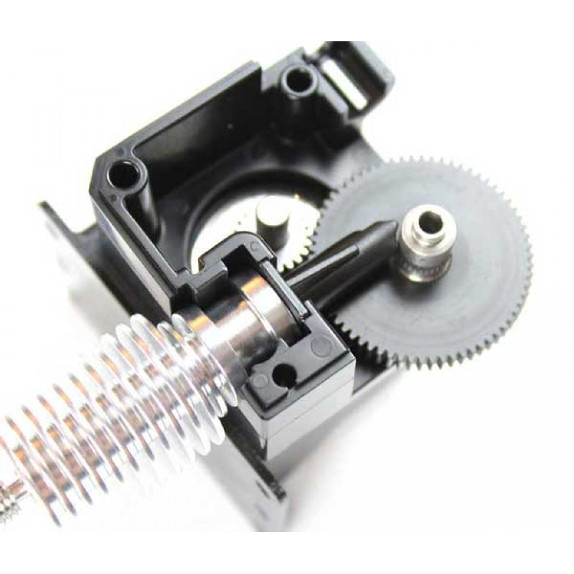
\includegraphics[width=\textwidth,cfbox=azul_marcos 4pt 0pt]{FOTOS/EXTRUSOR8}
		\caption*{\href{www.e3d-online.com}{{\footnotesize Titan Extruder - Precio aprox. 70\euro}}}
    \end{subfigure}
\end{figure}
\section{Consejos para un uso óptimo de FlexiSMART}
	\subsection{La retracción}
La retracción es una técnica usada en las impresoras 3D FFF/FDM para mejorar el acabado de las piezas. Consiste en ordenar al extrusor que retire unos centímetros de filamento cuando éste va a cambiar de posición para evitar el stringing o aparición de pequeños hilos de filamento entre diferentes partes de la pieza que se está imprimiendo.
\begin{figure}[H]
\centering
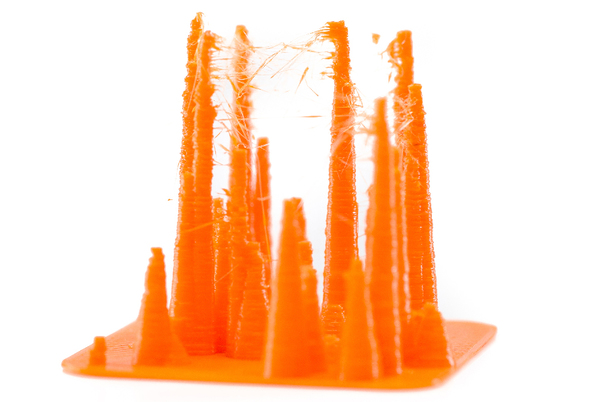
\includegraphics[width=0.5\textwidth,cfbox=azul_marcos 4pt 0pt]{FOTOS/RETRACCION1}
\caption*{Pieza con problema de stringing}
\end{figure}
Cuando se utilizan filamentos flexibles puede suceder que al intentar una retracción muy brusca el filamento se estire en lugar de retroceder. Por eso es muy recomendable utilizar unos parámetros de retracción diferentes a los utilizados con filamentos rígidos.
\\\\
Los 2 parámetros que podemos controlar en la retracción son el tamaño, o cantidad lineal en milimetros de filamento retraido, y la velocidad en mm/s de la operación. Ambos valores deben ser inferiores a los usados habitualmente. La forma óptima de calibrar estos valores es realizar pruebas para averiguar cuales son los valores máximos que soporta tu impresora al imprimir con FlexiSMART. En cualquier caso, como punto de partida puedes usar los valores recomendados por nosotros:
\begin{description}
\item [Tamaño de retracción:] 1.5 mm
\item [Velocidad de retracción:] 40 mm/s
\end{description}
Dependiendo de la impresora puede que sea necesario desactivar totalmente la retracción.
	\subsection{Impresión secuencial}
Al tratarse de un filamento flexible FlexiSMART tiene una viscosidad diferente a la de otros materiales cuando alcanza su temperatura de fusión. Por esto es más propenso a dejar pequeños hilos de filamento entre distintas partes de la pieza cuando el nozzle debe desplazarse de un punto a otro sin extruir.
\begin{figure}[H]
\centering
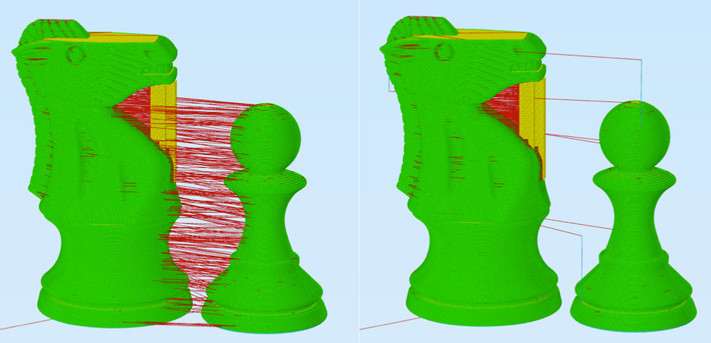
\includegraphics[width=0.5\textwidth,cfbox=azul_marcos 4pt 0pt]{FOTOS/SEQUENTIALPRINTING}
\caption*{Comparación de las rutas de impresión entre impresion simultanea y secuencial}
\end{figure}
Además, cuando se van a imprimir varias piezas distintas al mismo tiempo, estos pequeños hilos pueden crearse entre las piezas ya que el nozzle tiene que saltar de unas a otras constantemente.
\\\\
Como ya hemos comentado anteriormente este efecto puede reducirse haciendo uso de la retracción, pero es muy recomendable que además las distintas piezas se impriman de manera secuencial en vez de simultánea.
\\\\
Con impresión secuencial nos referimos a imprimir completamente una pieza antes de empezar a imprimir la siguiente.
\\\\
Esto se puede conseguir de 2 maneras diferentes:
\begin{itemize}
\item La opción trivial es imprimir sólo una pieza y una vez terminada repetir la misma impresión tantas veces como se quiera.
\item La segunda alternativa, más avanzada y con algunas limitaciones, es hacer uso de la opción que ofrecen algunos programas de laminado de imprimir una pieza cada vez. El tamaño máximo de las piezas que pueden ser impresas usando este método viene dado por las dimensiones del nozzle y la disposición de los ejes de la impresora. Recomendamos encarecidamente que te informes acerca de cómo usar estas opciones para no correr riesgo de dañar tu impresora. Puedes hacerlo a través de los siguientes enlaces:
\end{itemize}
\url{https://www.simplify3d.com/support/tutorials/multi-part-printing/}\\
\url{http://manual.slic3r.org/advanced/sequential-printing}\\
\url{https://ultimaker.com/en/community/3843-force-cura-to-print-objects-separately}
	\subsection{La primera capa}
La primera capa es el fundamento del resto de capas y puede marcar la diferencia entre una impresión satisfactoria y una impresión fallida.
\\\\
Al imprimir con FlexiSMART hay que poner una atención especial a la primera capa ya que, en ocasiones, una impresora nivelada correctamente para imprimir con PLA o ABS puede no estarlo para imprimir FlexiSMART de forma adecuada.
\\\\
Para saber si la impresora está correctamente nivelada hay que observar atentamente cómo la máquina realiza la primera capa.
\\\\
Si la primera capa parece translúcida significa que el nozzle está demasiado cerca de la plataforma y será necesario separarlo unas micras.
\\\\
En cambio si la primera capa parece despegarse o las pistas de material depositado presentan espacios sin plástico entre ellas será necesario acercar el nozzle unas micras a la plataforma.
\begin{figure}[H]
    \centering
    \begin{subfigure}[b]{0.3\textwidth}
        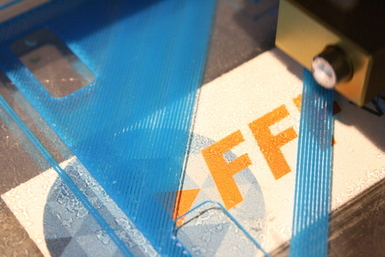
\includegraphics[width=\textwidth,cfbox=azul_marcos 3pt 0pt]{FOTOS/HOTENDALTO}
	\caption*{Nozzle demasiado lejos}
    \end{subfigure}
    ~ %add desired spacing between images, e. g. ~, \quad, \qquad, \hfill etc. 
      %(or a blank line to force the subfigure onto a new line)
    \begin{subfigure}[b]{0.3\textwidth}
        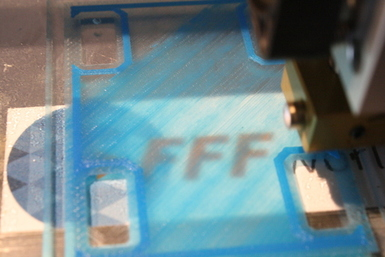
\includegraphics[width=\textwidth,cfbox=azul_marcos 3pt 0pt]{FOTOS/HOTENDBAJO}
	\caption*{Nozzle demasiado cerca}
    \end{subfigure}
    ~ %add desired spacing between images, e. g. ~, \quad, \qquad, \hfill etc. 
    %(or a blank line to force the subfigure onto a new line)
    \begin{subfigure}[b]{0.3\textwidth}
        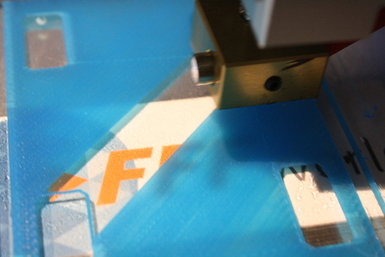
\includegraphics[width=\textwidth,cfbox=azul_marcos 3pt 0pt]{FOTOS/HOTENDPERFECTO}
	\caption*{Nozzle correctamente alineado}
    \end{subfigure}
\end{figure}
Este ajuste puede realizarse por software, ajustando el z-offset en el programa de laminado, o regulando el mecanismo de nivelación de la plataforma de impresión.
	\subsection{Consejos de laminación}
		\subsubsection{La altura de capa}
La altura de capa determina la calidad de la pieza y el tiempo de impresión.
\\\\
Utilizando un nozzle de 0.4 mm hemos comprobado que la altura de capa óptima es de 0.2 mm. Con esta altura de capa conseguirás capas fuertemente unidas con un acabado superficial excelente.
		\subsubsection{Los top layers y perimetros}
Las top layers y los perímetros son la envoltura lateral y superior de la pieza. El número adecuado de estos dependerá del infill y del uso que se le vaya a dar a la pieza.
\\\\
Con un infill alto, se puede reducir el número top-layers a 3 puesto que el relleno de la pieza les dará una buena base donde apoyarse. Utilizando unos valores de infill medios o bajos es recomendable aumentar el número de top-layers a 5 para asegurarse de que la parte superior de la pieza queda completamente sellada.
\\\\
Si la pieza va a sufrir deformaciones es recomendable aumentar el número de shells o perímetros horizontales. Aumentando el número de perímetros horizontales se evitará que las paredes de la pieza puedan cuartearse al realizar presión o tracción sobre ellas.
\\\\
Estas recomendaciones son válidas cuando se usa un nozzle de 0.4 mm y una altura de capa de 0.2 mm. Si el tamaño de nozzle o la altura de capa varía, el número de perímetros y top-layers óptimos también cambiará.
\\\\
Te invitamos a que realices tus propias pruebas y compartas con nosotros el resultado.
		\subsubsection{Influencia del infill en la flexibilidad}
La cantidad y el diseño del infill tiene una gran influencia en el grado de flexibilidad de las piezas impresas con FlexiSMART.
\\\\
Una pieza con un infill cercano al 100\% se comportará como un bloque de goma y puede ser una buena opción para piezas como silent-blocks o spacers.
\\\\
Utilizando un infill del 15\% obtendrás piezas blandas que podrán ser aplastadas y deformadas.
\\\\
El patrón de infill también afecta a la flexibilidad y no se comporta igual un infill rectilineo que un honeycomb (panel de abeja).  Te invitamos a que realices tus propias pruebas y elijas el que más se adecue a tu proyecto.
	\subsection{Utilización de un nozzle de mayor tamaño}
La mayor parte de las impresoras utilizan de serie un nozzle de 0.4 mm, un tamaño de nozzle que proporciona una buena proporción velocidad/resolución. FlexiSMART se imprime perfectamente con este tipo de nozzle sin embargo es conveniente hacer unas matizaciones.
\\\\
El tamaño del nozzle limita la cantidad de material que puede ser extruido por unidad de tiempo. Al utilizar filamentos rígidos este límite es mayor puesto que se puede aumentar la velocidad y el propio filamento soporta la presión extra necesaria para que el material salga por el nozzle. Con FlexiSMART sin embargo el filamento se comprime si esta presión es demasiado alta y, en general, debe ser impreso a velocidades menores.
\\\\
Por ello si quieres extruir FlexiSMART a velocidades elevadas es recomendable la utilización de un nozzle de mayor tamaño, a partir de 0.6 mm. Utilizando uno de estos nozzle podrás imprimir mucho más rápido, con alturas de capa superiores, sacrificando algo de resolución.
\section{¿Quieres apoyar nuestro proyecto?}
Todos los miembros FFF World amamos la impresión 3D y la comunidad maker. Nos sentimos afortunados de poder trabajar en proyectos donde podamos entregar nuestra pasión sincera. En el futuro, nos gustaría poder desarrollar más materiales, más colores, más formatos. En definitiva, nos gustaría poder hacer crecer nuestra empresa.
\\\\
Para ello, una de las principales acciones para ayudarnos, si quieres hacerlo y estás satisfecho con el filamento, es la de votarnos en Amazon con 5 estrellas.
\begin{figure}[H]
\centering

\includegraphics[width=0.5\textwidth,cfbox=azul_marcos 1pt 0pt]{FOTOS/AMAZON_FIVE_STARS}
\caption*{¡Muchas gracias!}
\end{figure}
\subsection{Another filaments with outstanding properties available now in Amazon}
\begin{description}
\item[FlexiSMART Tech:] Diseñado para resistir a la abrasión y al desgaste de impresiones técnicas.
\item[ABS Tech:] Efecto warping minimizado. Alto rendimiento en aplicaciones técnicas.
\item[PETG Tech:] Máxima resistencia mécanica. Resistente al contacto con el agua y los rayos UV. Apto para uso alimentario.
\item[FilaMETAL:] PLA con carga metálica no abrasiva que da un acabado metálico espectacular a tus impresiones.
\item[PC Tech:] Policarbonato con gran resistencia a la temperatura y con excelentes propiedades mecánicas.
\item[Nylon Tech:] Imprimible a baja temperatura. Resistencia a los golpes con cierto grado de flexibilidad.
\item[PVA Tech:] Filamento soluble en agua indicado para uso como material de soporte. Excelente compatibilidad con PLA.
\item[HIPS Tech:] Filamento soluble en limoneno indicado para uso como material de soporte. Buena resistencia mecánica y excelente compatibilidad con ABS.
\end{description}
%\section{Bibliografía}
%Esta guía no habría sido posible sin el conocimiento libre generado por la comunidad RepRap. Para la elaboración de esta guía se han %utilizado imágenes y contenido extraidos de los siguientes sitios web.
%\\\\
%\url{http://www.gyrobot.co.uk/blog/how-to-3d-print-with-flexible-filaments}\\
%\url{http://www.thingiverse.com/thing:1496895}\\
%\url{http://www.thingiverse.com/thing:247024}\\
%\url{http://www.thingiverse.com/thing:16319}\\
%\url{http://www.thingiverse.com/thing:779011}\\
%\url{http://www.thingiverse.com/thing:1102900}\\
%\url{http://www.thingiverse.com/thing:147705}\\
%\url{http://www.thingiverse.com/thing:222667}\\
%\url{http://www.thingiverse.com/thing:512338}\\
%\url{https://all3dp.com/common-3d-printing-problems-and-their-solutions/}\\
%\url{https://www.simplify3d.com/support/}\\
%\url{http://www.thingiverse.com/thing:508896}\\
%\url{http://www.thingiverse.com/thing:1187344}

\includepdf{PDF/ES_CONTRAPORTADA.pdf}
\end{document}
